% The analysis.
%%%%%%%%%%%%%%%

\section{Data analysis}

% Intro.
\subsection{Introduction}

The analysis consists of two parts.
The first is the single structure or ensemble analysis of the combined RDC and PCS alignment tensor for the non-moving paramagnetically aligned domain or rigid body.
The resultant alignment tensor and optimised paramagnetic Ln$^{3+}$ position is then used as input into the frame order analysis.


% The N-state model analysis scripts.
\subsection{The N-state model analysis scripts}
\label{sect: N-state model analysis scripts}

For determining the alignment tensor and paramagnetic Ln$^{3+}$ position from the RDC and PCS data, the N-state model or ensemble analysis should be used.
The script is:

\begin{lstlisting}
# Python imports.
from numpy import array

# relax imports.
from lib.physical_constants import NH_BOND_LENGTH_RDC


# Create a data pipe for all the data.
pipe.create('CaM N-dom', 'N-state')

# Load the CaM structure.
structure.read_pdb('2BE6_core_II_III.pdb', dir='../../../../structures/2BE6_superimpose/Ndom_II_III', set_mol_name=['CaM_A', 'IQ_A', 'Metals_A', 'CaM_B', 'IQ_B', 'Metals_B', 'CaM_C', 'IQ_C', 'Metals_C'])

# Load the spins.
structure.load_spins('@N', from_mols=['CaM_A', 'CaM_B', 'CaM_C'], mol_name_target='CaM', ave_pos=False)
structure.load_spins('@H', from_mols=['CaM_A', 'CaM_B', 'CaM_C'], mol_name_target='CaM', ave_pos=False)

# Select only the superimposed spins (skipping mobile residues :2-4,42,56-57,76-80, identified from model-free order parameters).
select.spin(':17-41,43-55,58-67', change_all=True)
select.display()

# Define the magnetic dipole-dipole relaxation interaction.
interatom.define(spin_id1='@N', spin_id2='@H', direct_bond=True)
interatom.set_dist(spin_id1='@N', spin_id2='@H', ave_dist=NH_BOND_LENGTH_RDC)
interatom.unit_vectors(ave=False)

# Set the nuclear isotope and element.
spin.isotope(isotope='15N', spin_id='@N')
spin.isotope(isotope='1H', spin_id='@H')

# The alignment data.
align_data = [
    ['dy', 'RDC_DY_111011_spinID.txt', 'PCS_DY_200911.txt', 900.00423401],
    ['tb', 'RDC_TB_111011_spinID.txt', 'PCS_TB_200911.txt', 900.00423381],
    ['tm', 'RDC_TM_111011_spinID.txt', 'PCS_TM_200911.txt', 900.00423431],
    ['er', 'RDC_ER_111011_spinID.txt', 'PCS_ER_200911.txt', 899.90423151],
    ['yb', 'RDC_YB_110112_spinID.txt', 'PCS_YB_211111.txt', 899.90423111],
    ['ho', 'RDC_HO_300512_spinID.txt', 'PCS_HO_300412.txt', 899.80423481]
]

# Loop over the alignments.
for i in range(len(align_data)):
    # Alias the data.
    TAG = align_data[i][0]
    RDC_FILE = align_data[i][1]
    PCS_FILE = align_data[i][2]
    FRQ = align_data[i][3]

    # RDCs.
    rdc.read(align_id=TAG, file=RDC_FILE, dir='../..', data_type='D', spin_id1_col=1, spin_id2_col=2, data_col=3, error_col=4)

    # PCSs.
    pcs.read(align_id=TAG, file=PCS_FILE, dir='../..', res_num_col=1, data_col=2, error_col=4, spin_id='@N')
    pcs.read(align_id=TAG, file=PCS_FILE, dir='../..', res_num_col=1, data_col=3, error_col=4, spin_id='@H')

    # The temperature.
    spectrometer.temperature(id=TAG, temp=303.0)

    # The frequency.
    spectrometer.frequency(id=TAG, frq=FRQ, units='MHz')

# The paramagnetic centre (average Ca2+ position).
ave = array([7.608, 5.402, 16.725]) + array([7.295, 4.684, 16.168]) + array([7.338, 5.275, 16.086])
ave = ave / 3
paramag.centre(pos=ave)

# Set up the model.
n_state_model.select_model('fixed')

# Tensor optimisation.
print("\n\n# Tensor optimisation.\n\n")
minimise.grid_search(inc=5)
minimise.execute('newton', constraints=False)
state.save('tensor_only_fit', force=True)

# Optimisation of everything.
paramag.centre(fix=False)
minimise.execute('bfgs', constraints=False)

# PCS structural noise.
print("\n\n# Tensor optimisation with PCS structural noise.\n\n")
pcs.structural_noise(rmsd=0.3, sim_num=10000, file='structural_noise.agr', force=True)

# Optimisation of everything.
paramag.centre(fix=False)
minimise.execute('bfgs', constraints=False)

# Monte Carlo simulations.
monte_carlo.setup(number=500)
monte_carlo.create_data()
monte_carlo.initial_values()
minimise.execute('bfgs', constraints=False)
monte_carlo.error_analysis()

# Show the tensors.
align_tensor.display()

# Q-factors.
rdc.calc_q_factors()
pcs.calc_q_factors()

# Correlation plots.
rdc.corr_plot(file="rdc_corr.agr", force=True)
pcs.corr_plot(file="pcs_corr.agr", force=True)

# Save the program state.
state.save('tensor_fit', force=True)
\end{lstlisting}

The calculation of the additional PCS error due to structural noise is very important for the subsequent frame order analysis.
A plot of such a calculation is shown in Figure~\ref{fig: CaM-IQ ABC X-ray structural noise}

% The structural noise figure.
% This is from CaM/align_data/CaM_IQ/tensors/camiq_abc_fit_whole.
\begin{figure}
  \centerline{
    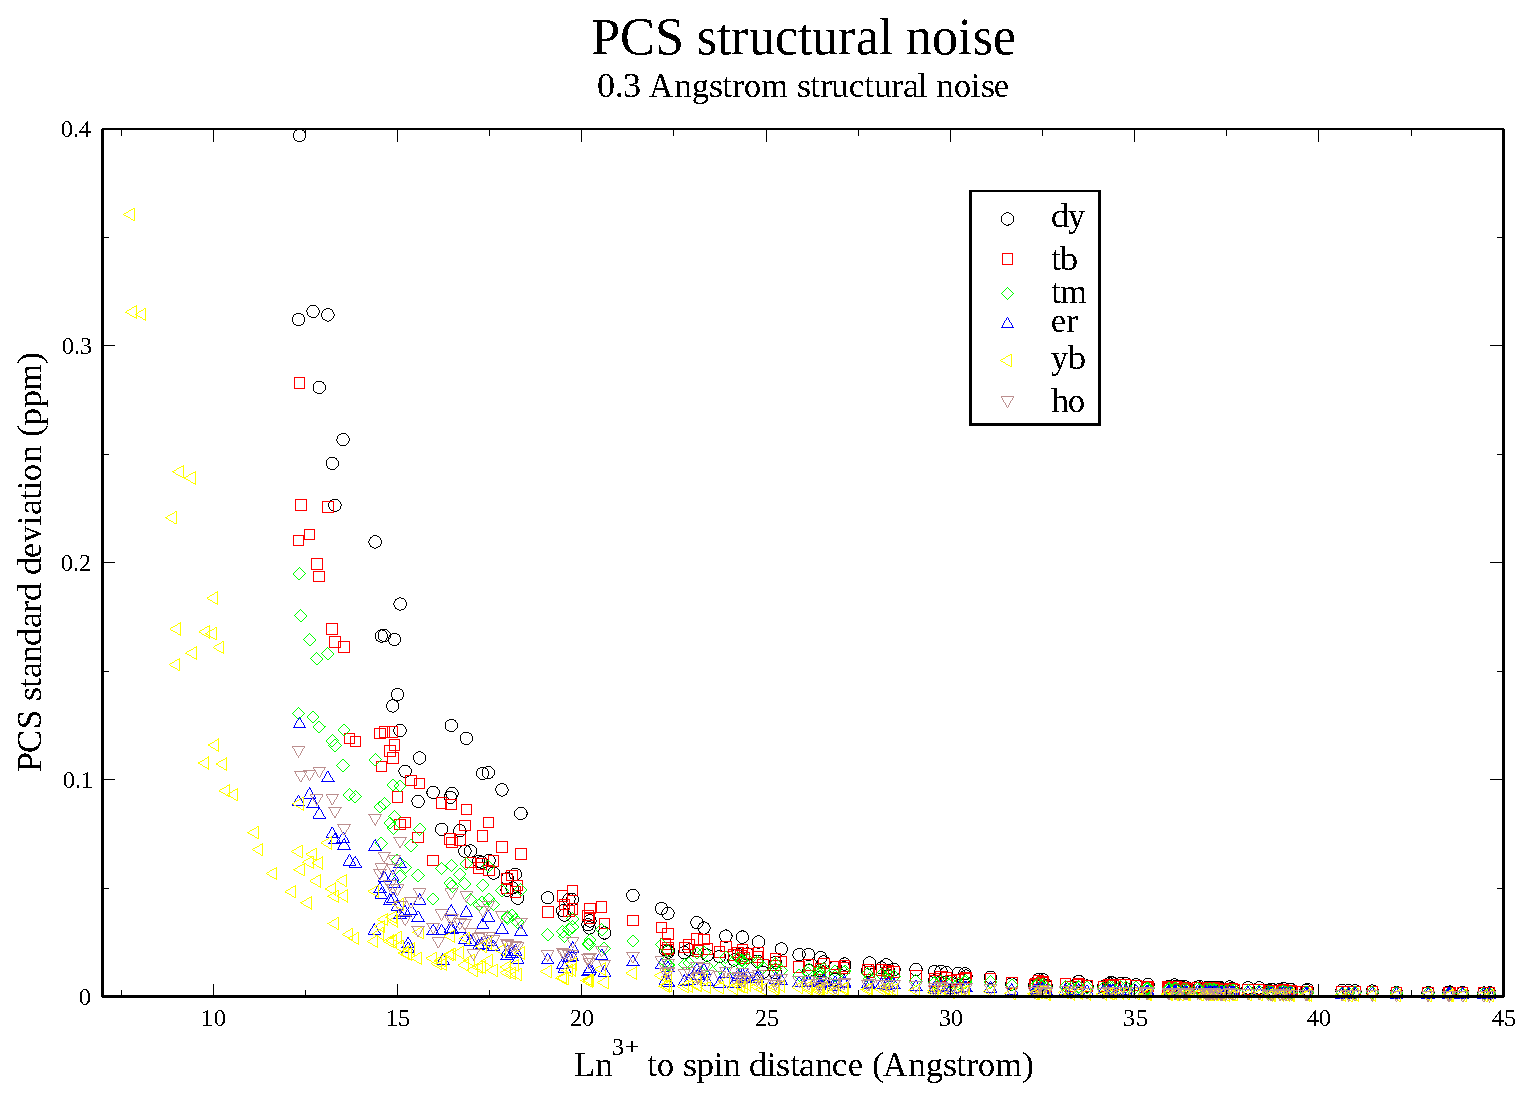
\includegraphics[width=\textwidth]{images/cam_iq_abc_whole_structural_noise}
  }
  \caption[Structural noise and the PCS error.]{
    Structural noise simulation using the 2BE6 CaM-IQ X-ray ABC ensemble as an example.
    The simulated structural error, with the atom position uncertainty set to 0.3~\AA, is an extra contribution to the measured PCS error.
    The PCS structural error is compared to the distance from the paramagnetic centre to illustrate the relationship between the two.
    The atomic positions were randomised 10,000 times with the lanthanide position assumed fixed, the PCS value back-calculated using a pre-fit alignment tensor, and the PCS standard deviations calculated.
  }
  \label{fig: CaM-IQ ABC X-ray structural noise}
\end{figure}


Statistics for the tensors, including the matrix or inter-tensor angles, the singular value decomposition (SVD) values and condition number, and a printout of the tensors for copying directly in the frame order analysis script, are obtained via the script:

\begin{lstlisting}
# Script for determining the tensor angles and SVD values of the CaM-IQ tensors.

# Load the state.
state.load('tensor_fit')

# Loop over the alignment tensors, producing a string of relax user function commands.
print("\nTensor strings for relax input:")
string = ""
for A in cdp.align_tensors:
    string += "align_tensor.init(tensor='%s', params=(%s, %s, %s, %s, %s), param_types=2)\n" % (A.name, A.Axx, A.Ayy, A.Axy, A.Axz, A.Ayz)
    string += "align_tensor.init(tensor='%s', params=(%s, %s, %s, %s, %s), param_types=2, errors=True)\n" % (A.name, A.Axx_err, A.Ayy_err, A.Axy_err, A.Axz_err, A.Ayz_err)
print(string)

# The matrix angles.
align_tensor.matrix_angles(basis_set=0)
align_tensor.matrix_angles(basis_set=1)

# The SVD analysis.
align_tensor.svd(basis_set=0)
align_tensor.svd(basis_set=1)
\end{lstlisting}


% The frame order analysis scripts.
\subsection{The frame order analysis scripts}
\label{sect: frame order analysis script}

The following is the example frame order analysis script located at \file{sample\_scripts/frame\_order/full\_analysis.py}:

\begin{lstlisting}
"""Script for black-box Frame Order analysis.

This is for the CaM-IQ data.

The free rotor pseudo-elliptic cone model is not used in this script as the cone X and Y opening angles cannot be differentiated with simply RDC and PCS data, hence this model is perfectly approximated by the free rotor isotropic cone.
"""

# Python module imports.
from numpy import array
from time import asctime, localtime

# relax module imports.
from auto_analyses.frame_order import Frame_order_analysis, Optimisation_settings


# Analysis variables.
#####################

# The frame order models to use.
MODELS = [
    'rigid',
    'rotor',
    'iso cone',
    'pseudo-ellipse',
    'iso cone, torsionless',
    'pseudo-ellipse, torsionless',
    'double rotor'
]

# The number of Monte Carlo simulations to be used for error analysis at the end of the protocol.
MC_NUM = 10

# Rigid model optimisation setup.
OPT_RIGID = Optimisation_settings()
OPT_RIGID.add_grid(inc=21, zoom=0)
OPT_RIGID.add_grid(inc=21, zoom=1)
OPT_RIGID.add_grid(inc=21, zoom=2)
OPT_RIGID.add_grid(inc=21, zoom=3)
OPT_RIGID.add_min(min_algor='simplex')

# PCS subset optimisation setup.
OPT_SUBSET = Optimisation_settings()
OPT_SUBSET.add_grid(inc=11, zoom=0, sobol_max_points=100)
OPT_SUBSET.add_grid(inc=11, zoom=1, sobol_max_points=100)
OPT_SUBSET.add_grid(inc=11, zoom=2, sobol_max_points=100)
OPT_SUBSET.add_min(min_algor='simplex', func_tol=1e-2, sobol_max_points=100)

# Full data set optimisation setup.
OPT_FULL = Optimisation_settings()
OPT_FULL.add_grid(inc=11, zoom=2, sobol_max_points=100)
OPT_FULL.add_grid(inc=11, zoom=3, sobol_max_points=100)
OPT_FULL.add_min(min_algor='simplex', func_tol=1e-2, sobol_max_points=100)
OPT_FULL.add_min(min_algor='simplex', func_tol=1e-3, sobol_max_points=1000)
OPT_FULL.add_min(min_algor='simplex', func_tol=1e-4, sobol_max_points=10000)

# Monte Carlo simulation optimisation setup.
OPT_MC = Optimisation_settings()
OPT_MC.add_min(min_algor='simplex', func_tol=1e-3, sobol_max_points=100)


# Set up the base data pipes.
#############################

# The data pipe bundle to group all data pipes.
PIPE_BUNDLE = "Frame Order (%s)" % asctime(localtime())

# Create the base data pipe containing only a subset of the PCS data.
SUBSET = "Data subset - " + PIPE_BUNDLE
pipe.create(pipe_name=SUBSET, pipe_type='frame order', bundle=PIPE_BUNDLE)

# Read the structures.
structure.read_pdb('2BE6_ndom_truncN.pdb', dir='../../../structures/2BE6_superimpose', set_mol_name='N-dom')
structure.read_pdb('2BE6_cdom_truncC.pdb', dir='../../../structures/2BE6_superimpose', set_mol_name='C-dom')

# Set up the 15N and 1H spins.
structure.load_spins(spin_id='@N', mol_name_target='CaM', ave_pos=False)
structure.load_spins(spin_id='@H', mol_name_target='CaM', ave_pos=False)
spin.isotope(isotope='15N', spin_id='@N')
spin.isotope(isotope='1H', spin_id='@H')

# Define the magnetic dipole-dipole relaxation interaction.
interatom.define(spin_id1='@N', spin_id2='@H', direct_bond=True)
interatom.set_dist(spin_id1='@N', spin_id2='@H', ave_dist=1.041 * 1e-10)
interatom.unit_vectors()

# Deselect mobile spins and vectors (from the CaM model-free order parameters from the BMRB).
deselect.spin(':2-4')
deselect.spin(':42')
deselect.spin(':56-57')
deselect.spin(':76-82')
deselect.spin(':114-117')
deselect.spin(':129-130')
deselect.spin(':146-148')
deselect.interatom(':2-4')
deselect.interatom(':42')
deselect.interatom(':56-57')
deselect.interatom(':76-82')
deselect.interatom(':114-117')
deselect.interatom(':129-130')
deselect.interatom(':146-148')

# The lanthanides and data files.
ln = ['dy', 'tb', 'tm', 'er', 'yb', 'ho']
pcs_files = [
    'PCS_DY_200911.txt',
    'PCS_TB_200911.txt',
    'PCS_TM_200911.txt',
    'PCS_ER_200911.txt',
    'PCS_YB_211111.txt',
    'PCS_HO_300412.txt'
]
pcs_files_subset = [
    'PCS_DY_200911_subset.txt',
    'PCS_TB_200911_subset.txt',
    'PCS_TM_200911_subset.txt',
    'PCS_ER_200911_subset.txt',
    'PCS_YB_211111_subset.txt',
    'PCS_HO_300412_subset.txt'
]
rdc_files = [
    'RDC_DY_111011_spinID.txt',
    'RDC_TB_111011_spinID.txt',
    'RDC_TM_111011_spinID.txt',
    'RDC_ER_111011_spinID.txt',
    'RDC_YB_110112_spinID.txt',
    'RDC_HO_300512_spinID.txt'
]

# The spectrometer frequencies for Luigi's measurements (matching the above lanthanide ordering, taken from the acqus SFO1 parameter).
pcs_frq = [
    701.2533001,    # Dy3+.
    701.2533002,    # Tb3+.
    701.2533005,    # Tm3+.
    701.2533003,    # Er3+.
    701.2533004,    # Yb3+.
    701.2533005     # Ho3+.
]
rdc_frq = [
    900.00423401,   # Dy3+.
    900.00423381,   # Tb3+.
    900.00423431,   # Tm3+.
    899.90423151,   # Er3+.
    899.90423111,   # Yb3+.
    899.80423481,   # Ho3+.
]

# Loop over the alignments.
for i in range(len(ln)):
    # Load the RDCs.
    rdc.read(align_id=ln[i], file=rdc_files[i], dir='../../../align_data/CaM_IQ/', spin_id1_col=1, spin_id2_col=2, data_col=3, error_col=4)

    # The 1H PCS (only a subset of ~5 spins for fast initial optimisations).
    pcs.read(align_id=ln[i], file=pcs_files_subset[i], dir='../../../align_data/CaM_IQ/', res_num_col=1, data_col=3, error_col=4, spin_id='@H')

    # The temperature and field strength.
    spectrometer.temperature(id=ln[i], temp=303.0)
    spectrometer.frequency(id=ln[i], frq=rdc_frq[i], units="MHz")

# Set up the tensors from the CaM-IQ ABC :6-74@N,CA,C,O N-state model fit.
align_tensor.init(tensor='Dy N-dom', align_id='dy', params=(-0.000895122969134, 0.000200206126748, 0.000350783562498, 0.000789321179176, -0.000185956794915), param_types=2)
align_tensor.init(tensor='Dy N-dom', align_id='dy', params=(1.2293468401e-05, 1.74966511177e-05, 1.07296910627e-05, 1.21471537359e-05, 9.98472771055e-06), param_types=2, errors=True)
align_tensor.init(tensor='Tb N-dom', align_id='tb', params=(-0.000386773980249, -0.000252229451755, 0.000289345115245, 0.00077454551221, -0.000411564842864), param_types=2)
align_tensor.init(tensor='Tb N-dom', align_id='tb', params=(9.08568851197e-06, 1.25046911688e-05, 9.13279347879e-06, 8.66699785438e-06, 8.17084290029e-06), param_types=2, errors=True)
align_tensor.init(tensor='Tm N-dom', align_id='tm', params=(0.000138832563763, 0.00019276873546, -0.000401761891364, -0.00053984778662, 0.000385156710458), param_types=2)
align_tensor.init(tensor='Tm N-dom', align_id='tm', params=(7.45028293534e-06, 1.15087527652e-05, 7.80160598908e-06, 7.48687231235e-06, 8.44077530542e-06), param_types=2, errors=True)
align_tensor.init(tensor='Er N-dom', align_id='er', params=(0.00013266928235, 6.08491225722e-05, -0.000249892897607, -0.000344865388853, 0.000118692962249), param_types=2)
align_tensor.init(tensor='Er N-dom', align_id='er', params=(6.24728334522e-06, 8.68937486363e-06, 7.96726504939e-06, 6.43064935791e-06, 1.00354375045e-05), param_types=2, errors=True)
align_tensor.init(tensor='Yb N-dom', align_id='yb', params=(0.000150564392882, -7.59743643441e-05, -0.00013958907081, -0.000188379895441, 0.000102722198261), param_types=2)
align_tensor.init(tensor='Yb N-dom', align_id='yb', params=(4.42731599871e-06, 5.1565091874e-06, 5.18051425981e-06, 3.9225664592e-06, 4.49007020445e-06), param_types=2, errors=True)
align_tensor.init(tensor='Ho N-dom', align_id='ho', params=(-0.000307522207243, 2.76511812842e-05, 0.000152789357344, 0.000307999279733, -0.000235201851074), param_types=2)
align_tensor.init(tensor='Ho N-dom', align_id='ho', params=(6.56971189673e-06, 1.0420422445e-05, 8.05282585054e-06, 7.42469124453e-06, 7.25413636142e-06), param_types=2, errors=True)

# Define the domains.
domain(id='N', spin_id=":1-78")
domain(id='C', spin_id=":80-148")

# The tensor domains and reductions.
full = ['Dy N-dom', 'Tb N-dom', 'Tm N-dom', 'Er N-dom', 'Yb N-dom', 'Ho N-dom']
red =  ['Dy C-dom', 'Tb C-dom', 'Tm C-dom', 'Er C-dom', 'Yb C-dom', 'Ho C-dom']
ids = ['dy', 'tb', 'tm', 'er', 'yb', 'ho']
for i in range(len(full)):
    # Initialise the reduced tensors (fitted during optimisation).
    align_tensor.init(tensor=red[i], align_id=ids[i], params=(0, 0, 0, 0, 0))

    # Set the domain info.
    align_tensor.set_domain(tensor=full[i], domain='N')
    align_tensor.set_domain(tensor=red[i], domain='C')

    # Specify which tensor is reduced.
    align_tensor.reduction(full_tensor=full[i], red_tensor=red[i])

# Set the reference domain.
frame_order.ref_domain('N')

# Set the initial pivot point.
pivot = array([ 21.863, 5.270, 5.934])
frame_order.pivot(pivot, fix=False)

# Set the paramagnetic centre position.
paramag.centre(pos=[6.518, 8.520, 13.767])

# Duplicate the PCS data subset data pipe to create a data pipe containing all the PCS data.
DATA = "Data - " + PIPE_BUNDLE
pipe.copy(pipe_from=SUBSET, pipe_to=DATA, bundle_to=PIPE_BUNDLE)
pipe.switch(DATA)

# Load the complete PCS data into the already filled data pipe.
for i in range(len(ln)):
    # The 15N PCS.
    pcs.read(align_id=ln[i], file=pcs_files[i], dir='../../../align_data/CaM_IQ/', res_num_col=1, data_col=2, error_col=4, spin_id='@N')

    # The 1H PCS.
    pcs.read(align_id=ln[i], file=pcs_files[i], dir='../../../align_data/CaM_IQ/', res_num_col=1, data_col=3, error_col=4, spin_id='@H')


# Execution.
############

# Do not change!
Frame_order_analysis(data_pipe_full=DATA, data_pipe_subset=SUBSET, pipe_bundle=PIPE_BUNDLE, results_dir=None, opt_rigid=OPT_RIGID, opt_subset=OPT_SUBSET, opt_full=OPT_FULL, opt_mc=OPT_MC, mc_sim_num=MC_NUM, models=MODELS)
\end{lstlisting}

Once this analysis has been completed then, a refinement step is required.
This is due to the low amount of motion in the system which causes the pivot point to be less well defined and hence strongly affected by artifacts of discrete sampling of a continuous and uniform distribution.
The collapse of certain cone open half-angles and torsion angles to zero also causes the number of Sobol' points $N$ to sometimes be zero.
The refinement script is:

\begin{lstlisting}
"""Script for black-box Frame Order analysis.

This is for the CaM-IQ data.

The free rotor pseudo-elliptic cone model is not used in this script as the cone X and Y opening angles cannot be differentiated with simply RDC and PCS data, hence this model is perfectly approximated by the free rotor isotropic cone.
"""

# Python module imports.
from time import asctime, localtime

# relax module imports.
from auto_analyses.frame_order import Frame_order_analysis, Optimisation_settings


# Analysis variables.
#####################

# The frame order models to use.
MODELS = [
    'rigid',
    'rotor',
    'iso cone',
    'pseudo-ellipse',
    'iso cone, torsionless',
    'pseudo-ellipse, torsionless',
    'double rotor'
]

# The number of Monte Carlo simulations to be used for error analysis at the end of the protocol.
MC_NUM = 10

# Full data set optimisation setup.
OPT_FULL = Optimisation_settings()
OPT_FULL.add_min(min_algor='simplex', func_tol=1e-4, quad_int=True)

# Monte Carlo simulation optimisation setup.
OPT_MC = Optimisation_settings()
OPT_MC.add_min(min_algor='simplex', func_tol=1e-3, quad_int=True)


# Set up the base data pipes.
#############################

# The data pipe bundle to group all data pipes.
PIPE_BUNDLE = "Frame Order (%s)" % asctime(localtime())


# Execution.
############

# Do not change!
Frame_order_analysis(pipe_bundle=PIPE_BUNDLE, results_dir='refinement', pre_run_dir='.', opt_full=OPT_FULL, opt_mc=OPT_MC, mc_sim_num=MC_NUM, models=MODELS)
\end{lstlisting}



% Computation times.
%~~~~~~~~~~~~~~~~~~~

\subsection{Computation times}

It should be noted that computation times are currently very long, in the order of months.
This depends on the models chosen, the amount and quality of the input data, and the refinement step.
This is due to the numeric integration for the PCS data.
Calculations can range from one to six months on a very fast computer.
Unfortunately parallelization was not possible, but multiple analyses can be performed simultaneously on multiple core or multiple CPU systems.
A dedicated machine with a reliable UPS system is highly recommended.
